\documentclass[11pt,]{article}
\usepackage[left=1in,top=1in,right=1in,bottom=1in]{geometry}
\newcommand*{\authorfont}{\fontfamily{phv}\selectfont}
\usepackage[]{mathpazo}


  \usepackage[T1]{fontenc}
  \usepackage[utf8]{inputenc}



\usepackage{abstract}
\renewcommand{\abstractname}{}    % clear the title
\renewcommand{\absnamepos}{empty} % originally center

\renewenvironment{abstract}
 {{%
    \setlength{\leftmargin}{0mm}
    \setlength{\rightmargin}{\leftmargin}%
  }%
  \relax}
 {\endlist}

\makeatletter
\def\@maketitle{%
  \newpage
%  \null
%  \vskip 2em%
%  \begin{center}%
  \let \footnote \thanks
    {\fontsize{18}{20}\selectfont\raggedright  \setlength{\parindent}{0pt} \@title \par}%
}
%\fi
\makeatother




\setcounter{secnumdepth}{3}

\usepackage{longtable,booktabs}

\usepackage{graphicx,grffile}
\makeatletter
\def\maxwidth{\ifdim\Gin@nat@width>\linewidth\linewidth\else\Gin@nat@width\fi}
\def\maxheight{\ifdim\Gin@nat@height>\textheight\textheight\else\Gin@nat@height\fi}
\makeatother
% Scale images if necessary, so that they will not overflow the page
% margins by default, and it is still possible to overwrite the defaults
% using explicit options in \includegraphics[width, height, ...]{}
\setkeys{Gin}{width=\maxwidth,height=\maxheight,keepaspectratio}

\title{Estudio ecológico de la familia Malvacease  }



\author{\Large Carolain Pérez Ureña\vspace{0.05in} \newline\normalsize\emph{Estudiante, Universidad Autónoma de Santo Domingo (UASD)}  }


\date{}

\usepackage{titlesec}

\titleformat*{\section}{\normalsize\bfseries}
\titleformat*{\subsection}{\normalsize\itshape}
\titleformat*{\subsubsection}{\normalsize\itshape}
\titleformat*{\paragraph}{\normalsize\itshape}
\titleformat*{\subparagraph}{\normalsize\itshape}

\titlespacing{\section}
{0pt}{36pt}{0pt}
\titlespacing{\subsection}
{0pt}{36pt}{0pt}
\titlespacing{\subsubsection}
{0pt}{36pt}{0pt}





\newtheorem{hypothesis}{Hypothesis}
\usepackage{setspace}

\makeatletter
\@ifpackageloaded{hyperref}{}{%
\ifxetex
  \PassOptionsToPackage{hyphens}{url}\usepackage[setpagesize=false, % page size defined by xetex
              unicode=false, % unicode breaks when used with xetex
              xetex]{hyperref}
\else
  \PassOptionsToPackage{hyphens}{url}\usepackage[unicode=true]{hyperref}
\fi
}

\@ifpackageloaded{color}{
    \PassOptionsToPackage{usenames,dvipsnames}{color}
}{%
    \usepackage[usenames,dvipsnames]{color}
}
\makeatother
\hypersetup{breaklinks=true,
            bookmarks=true,
            pdfauthor={Carolain Pérez Ureña (Estudiante, Universidad Autónoma de Santo Domingo (UASD))},
             pdfkeywords = {palabra clave 1, palabra clave 2},  
            pdftitle={Estudio ecológico de la familia Malvacease},
            colorlinks=true,
            citecolor=blue,
            urlcolor=blue,
            linkcolor=magenta,
            pdfborder={0 0 0}}
\urlstyle{same}  % don't use monospace font for urls

% set default figure placement to htbp
\makeatletter
\def\fps@figure{htbp}
\makeatother

\usepackage{pdflscape} \newcommand{\blandscape}{\begin{landscape}}
\newcommand{\elandscape}{\end{landscape}} \usepackage{float}
\floatplacement{figure}{H}
\newcommand{\beginsupplement}{ \setcounter{table}{0} \renewcommand{\thetable}{S\arabic{table}} \setcounter{figure}{0} \renewcommand{\thefigure}{S\arabic{figure}} }


% add tightlist ----------
\providecommand{\tightlist}{%
\setlength{\itemsep}{0pt}\setlength{\parskip}{0pt}}

\begin{document}
	
% \pagenumbering{arabic}% resets `page` counter to 1 
%
% \maketitle

{% \usefont{T1}{pnc}{m}{n}
\setlength{\parindent}{0pt}
\thispagestyle{plain}
{\fontsize{18}{20}\selectfont\raggedright 
\maketitle  % title \par  

}

{
   \vskip 13.5pt\relax \normalsize\fontsize{11}{12} 
\textbf{\authorfont Carolain Pérez Ureña} \hskip 15pt \emph{\small Estudiante, Universidad Autónoma de Santo Domingo (UASD)}   

}

}






\vskip 6.5pt


\noindent  \section{Introducción}\label{introducciuxf3n}

La Ecología es una disciplica científica dentro de las ciencias
biológicas y físicas basada en el estudio de la relación entre los
organismos y su medio ambiente.La relación incluye interacciones con el
mundo físico, así como también con miembros de la misma y de otras
especies.(Smith \& Leo Smith, 2007) Desde esta perspectiva los estudios
ecológicos

(Bishop, 1995; Sun, Rosin, Martin, \& Langbein, 2007)

\begin{figure}
\centering
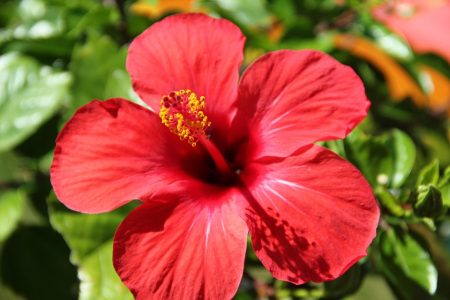
\includegraphics[width=0.50000\textwidth]{Hibiscus-Malvaceae.jpg}
\caption{Flor}
\end{figure}

\begin{longtable}[]{@{}lllll@{}}
\toprule
12 & 34 & 56 & 77 & 23\tabularnewline
\midrule
\endhead
67 & 85 & 234 & 86 & 89\tabularnewline
93 & 45 & texto prueba & &\tabularnewline
& & & &\tabularnewline
\bottomrule
\end{longtable}

\begin{figure}
\centering
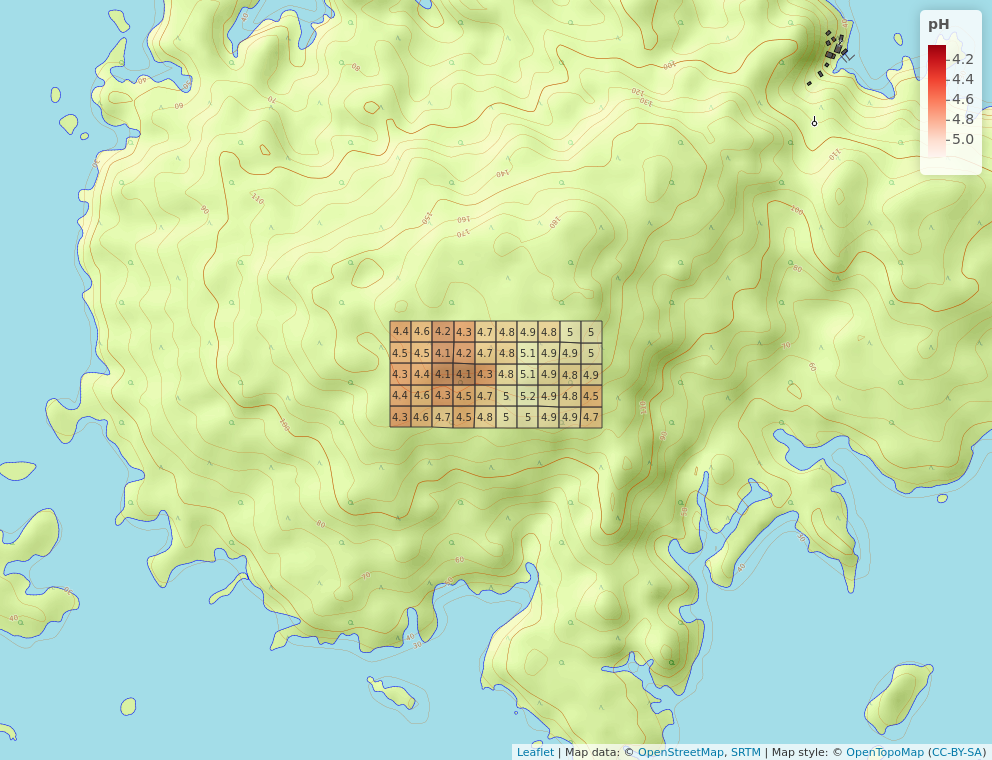
\includegraphics{mapa_cuadros_ph.png}
\caption{Districución del PH por cuadros de 1 Ha}
\end{figure}

\begin{figure}
\centering
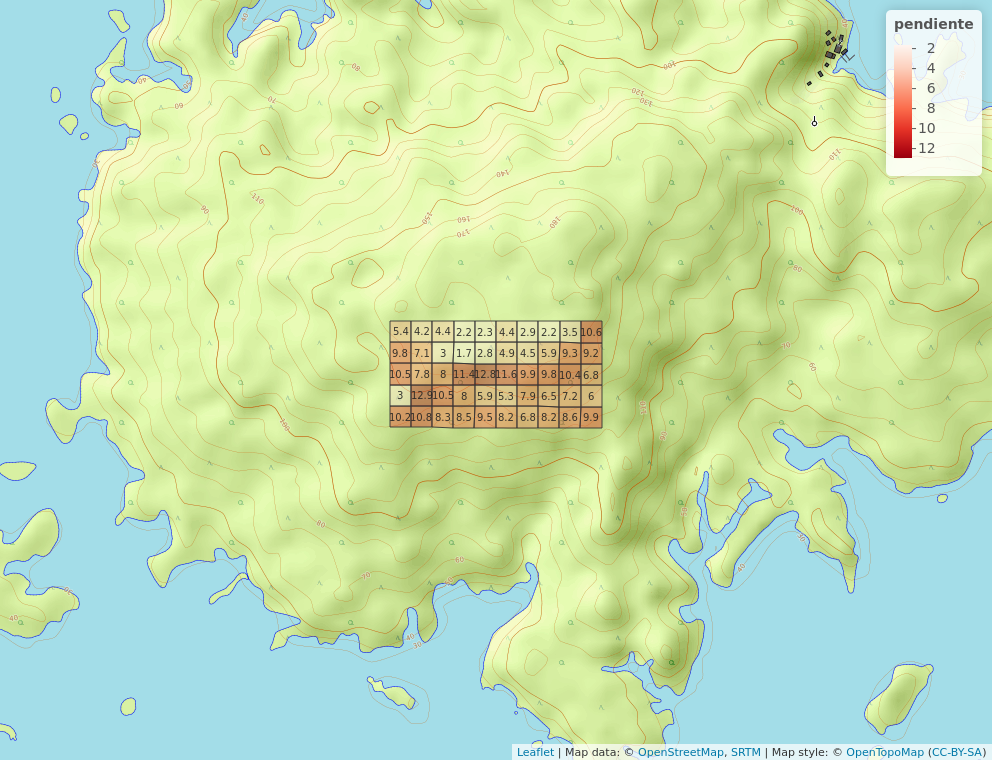
\includegraphics{mapa_cuadros_pendiente.png}
\caption{Districución de las pendientes en grados por cuadros de 1
Ha\label{fig:mapa_cuadros_pendiente}}
\end{figure}

\section{Metodología}\label{metodologuxeda}

\ldots

\section{Resultados}\label{resultados}

\ldots

\section{Discusión}\label{discusiuxf3n}

\section{Agradecimientos}\label{agradecimientos}

\section{Información de soporte}\label{informaciuxf3n-de-soporte}

\ldots

\section{\texorpdfstring{\emph{Script}
reproducible}{Script reproducible}}\label{script-reproducible}

\ldots

\section*{Referencias}\label{referencias}
\addcontentsline{toc}{section}{Referencias}

\hypertarget{refs}{}
\hypertarget{ref-bishop1995drainage}{}
Bishop, P. (1995). Drainage rearrangement by river capture, beheading
and diversion. \emph{Progress in Physical Geography}, \emph{19}(4),
449--473.

\hypertarget{ref-smith2007ecologia}{}
Smith, T. M., \& Leo Smith, R. (2007). \emph{Ecología}. Pearson
Educación,

\hypertarget{ref-sun2007fast}{}
Sun, X., Rosin, P., Martin, R., \& Langbein, F. (2007). Fast and
effective feature-preserving mesh denoising. \emph{IEEE Transactions on
Visualization \& Computer Graphics}, (5), 925--938.




\newpage
\singlespacing 
\end{document}
